\documentclass{article}

\usepackage{hyperref}
\usepackage[T1]{fontenc}
\usepackage{graphicx}
\usepackage{float}
\usepackage[utf8]{inputenc}
\usepackage{amsmath}


\title{%
Laboratorium 8\\
  \huge Rozwiązywanie równań nieliniowych}
\author{Mateusz Król}
\date{07/05/2024 r.}

\begin{document}
\maketitle

 
\section*{Zadanie 1.}
\textbf{Dla poniższych funkcji i punktów początkowych metoda 
\textit{Newton}'a
zawodzi. Wyjaśnij dlaczego. Następnie znajdź pierwiastki.
$$f_1(x) = x^3-5x,\ x_0=1$$
$$f_2(x) = x^3-3x+1,\ x_0=1$$
$$f_3(x) = 2-x^5,\ x_0=0.01$$
$$f_4(x) = x^4-4.29x^2-5.29,\ x_0=0.8$$} \\
\null\quad
Wykorzystałem funkcję \textit{scipy.optimize.newton} z modułu
\textit{SciPy}. \\\\
Dla funkcji $f_1$ metoda \textit{Newton}'a działa - zwraca prawdziwy
pierwiastek ($\approx 4.7 \cdot 10^{-24} \approx 0$). W celu zwrócenia
innego pierwiastka, możnaby zmienić wartość początkową na bliższą
odpowiedniej wartości (np. $2$). \\\\
Dla reszty funkcji metoda \textit{Newton}'a nie działa: \\\\
Dla funkcji $f_2$ odpowiednim $x_0$ byłoby $1.5$, gdyż wartość $1$ jest
ekstremum lokalnym. \\
Dla funkcji $f_3$ lepszym wyborem $x_0$ byłoby $1.1$, gdyż wartość
$0.01$ jest zbyt blisko 0, gdzie funkcja jest na tyle płaska, że
wartość przybliżana zbyt wolno zbiega do prawdziwego pierwiastka. \\
Dla funkcji $f_3$ odpowiednim $x_0$ byłoby $2.0$ - wartość bliżej 
prawdziwego pierwiastka. \\\\

\section*{Zadanie 2.}
\textbf{Dane jest równanie: $$f(x)=x^2-3x+2=0$$
Każda z następujących funkcji definiuje równoważny schemat iteracyjny:
$$g_1(x)=\frac{(x^2+2)}{3}$$
$$g_2(x)=\sqrt[]{3x-2}$$
$$g_3(x)=3-\frac{2}{x}$$
$$g_4(x)=\frac{(x^2-2)}{2x-3}.$$
}
\\\\
Tabela z wartościami rzędów zbieżności schematów iteracyjnych 
odpowiadających funkcjom $g_i(x)$:
\begin{center}
  \begin{tabular}{c c} 
   Function & Order of convergence\\
   $g_1$ & $\approx 1.33$\\
   $g_2$ & $\approx 0.82$\\
   $g_3$ & $\approx 0.67$\\
   $g_4$ & $\approx 0.67$
  \end{tabular}
\end{center}
Wykres przedstawiający porównanie wartości błędów względnych w zależności od liczby
iteracji:
\begin{figure}[H]
  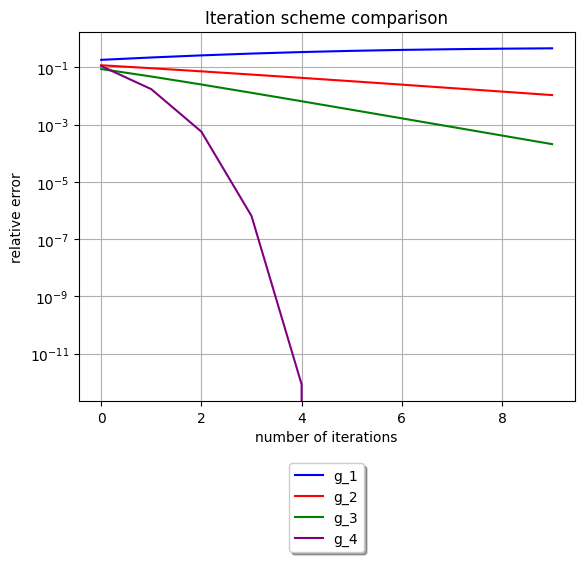
\includegraphics[width=\linewidth]{figures/iteration.png}
\end{figure}


\section*{Zadanie 3.}
\textbf{Napisz schemat iteracji wg metody Newtona dla każdego z nastę-
pujących równań nieliniowych:}

\section*{Zadanie 4.}
\textbf{Napisz schemat iteracji wg metody Newtona dla następującego
układu równań nieliniowych:}


\subsection*{Wnioski}
\null\quad 

\end{document}